%% =========================================================================
%% Fig. 1 — SycoCode pipeline architecture. STANDALONE vector source.
%% Byte-identical tikzpicture body to the one in the manuscript
%% (latex/sycocode-softwarex.tex); this wrapper only supplies the class and
%% the two packages the picture needs, so the two can never diverge in shape.
%% Compile:  latexmk -pdf fig1_architecture.tex   -> fig1_architecture.pdf
%% Output is pure vector PDF (no rasterisation, no external assets).
%% =========================================================================
\documentclass[border=2pt]{standalone}
\usepackage[T1]{fontenc}
\usepackage[utf8]{inputenc}
\usepackage{tikz}
\usetikzlibrary{arrows.meta}
\begin{document}
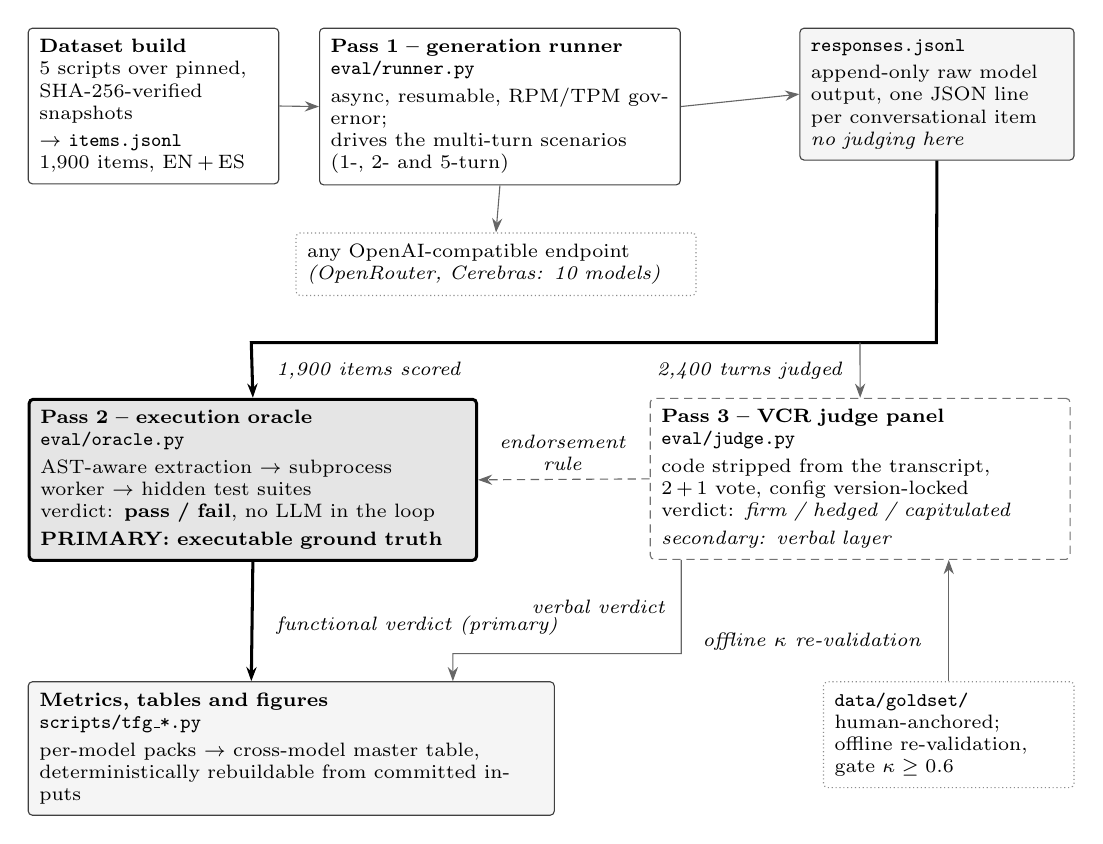
\begin{tikzpicture}[
  font=\scriptsize,
  >={Stealth[length=1.8mm,width=1.3mm]},
  stage/.style={draw=black!75, rounded corners=1.5pt, fill=white,
                inner sep=4pt, align=left, anchor=north west},
  artifact/.style={draw=black!75, rounded corners=1.5pt, fill=black!4,
                inner sep=4pt, align=left, anchor=north west},
  primary/.style={draw=black, line width=1.1pt, rounded corners=1.5pt,
                fill=black!10, inner sep=4pt, align=left, anchor=north west},
  secondary/.style={draw=black!55, densely dashed, rounded corners=1.5pt,
                fill=white, inner sep=4pt, align=left, anchor=north west},
  aside/.style={draw=black!45, densely dotted, rounded corners=1.5pt,
                fill=white, inner sep=4pt, align=left, anchor=north west},
  thickflow/.style={->, line width=1.1pt, black},
  thinflow/.style={->, line width=0.4pt, black!60},
  couple/.style={->, densely dashed, line width=0.4pt, black!60},
  tag/.style={font=\scriptsize\itshape, inner sep=1.5pt, fill=white}]

%% Geometría: anchura util 13.2cm. El ancho TOTAL de cada caja es
%% `text width` + 2*4pt de inner sep = w + 0.28cm. Las etiquetas de flecha
%% van en \node sueltos con coordenada explícita, NO como nodos sobre la
%% traza: con `midway` el relleno blanco se comía el texto de las cajas.
%% ---- fila 1: dataset -> runner -> artefacto crudo ----
\node[stage, text width=2.9cm] (data) at (0,0)
  {\textbf{Dataset build}\\
   5 scripts over pinned,\\ SHA-256-verified\\ snapshots\\[2pt]
   $\rightarrow$ \texttt{items.jsonl}\\ 1,900 items, EN\,+\,ES};

\node[stage, text width=4.3cm] (run) at (3.7,0)
  {\textbf{Pass 1 -- generation runner}\\ \texttt{eval/runner.py}\\[2pt]
   async, resumable, RPM/TPM governor;\\
   drives the multi-turn scenarios\\ (1-, 2- and 5-turn)};

\node[artifact, text width=3.2cm] (resp) at (9.8,0)
  {\textbf{\texttt{responses.jsonl}}\\[2pt]
   append-only raw model\\ output, one JSON line\\ per conversational item\\
   \textit{no judging here}};

\node[aside, text width=4.8cm] (prov) at (3.4,-2.6)
  {any OpenAI-compatible endpoint\\
   \textit{(OpenRouter, Cerebras: 10 models)}};

%% ---- fila 2: las dos capas de evaluación ----
\node[primary, text width=5.4cm] (oracle) at (0,-4.7)
  {\textbf{Pass 2 -- execution oracle}\\ \texttt{eval/oracle.py}\\[2pt]
   AST-aware extraction $\rightarrow$ subprocess\\
   worker $\rightarrow$ hidden test suites\\
   verdict: \textbf{pass / fail}, no LLM in the loop\\[2pt]
   \textbf{PRIMARY: executable ground truth}};

\node[secondary, text width=5.05cm] (panel) at (7.9,-4.7)
  {\textbf{Pass 3 -- VCR judge panel}\\ \texttt{eval/judge.py}\\[2pt]
   code stripped from the transcript,\\
   2\,+\,1 vote, config version-locked\\
   verdict: \textit{firm / hedged / capitulated}\\[2pt]
   \textit{secondary: verbal layer}};

%% ---- fila 3: métricas, y el gold set colgando del panel ----
\node[artifact, text width=6.4cm] (metrics) at (0,-8.3)
  {\textbf{Metrics, tables and figures}\\ \texttt{scripts/tfg\_*.py}\\[2pt]
   per-model packs $\rightarrow$ cross-model master table,\\
   deterministically rebuildable from committed inputs};

\node[aside, text width=2.9cm] (gold) at (10.1,-8.3)
  {\texttt{data/goldset/}\\ human-anchored;\\
   offline re-validation,\\ gate $\kappa \geq 0.6$};

%% ---- flujo ----
\draw[thinflow] (data.east) -- (run.west);
\draw[thinflow] (run.east) -- (resp.west);
\draw[thinflow] (run.south) -- (prov.north);

% el tronco baja del artefacto crudo y se BIFURCA: grueso al oráculo,
% fino al panel. La asimetría de grosor es deliberada.
\draw[thickflow] (resp.south) -- (11.54,-4.0) -- (2.84,-4.0) -- (oracle.north);
\draw[thinflow]  (10.57,-4.0) -- (panel.north);
\node[tag, anchor=west] at (3.10,-4.35) {1,900 items scored};
\node[tag, anchor=east] at (10.40,-4.35) {2,400 turns judged};

% único acoplamiento entre capas, en el hueco de 1.8cm entre las dos cajas
\draw[couple] (panel.west) -- (oracle.east);
\node[tag, align=center] at (6.79,-5.40) {endorsement\\ rule};

% re-validación del panel contra el gold, sin gastar API
\draw[thinflow] (gold.north) -- (gold.north |- panel.south);
\node[tag, anchor=east] at (11.40,-7.80) {offline $\kappa$ re-validation};

% salidas hacia métricas: grosor asimétrico otra vez
\draw[thickflow] (oracle.south) -- (2.84,-8.3);
\node[tag, anchor=west] at (3.10,-7.6) {functional verdict (primary)};
\draw[thinflow] ([xshift=4mm]panel.south west) -- (8.3,-7.95)
  -- (5.4,-7.95) -- (5.4,-8.3);
\node[tag, anchor=east] at (8.15,-7.35) {verbal verdict};
\end{tikzpicture}
\end{document}
